% Этот шаблон документа разработан в 2014 году
% Данилом Фёдоровых (danil@fedorovykh.ru) 
% для использования в курсе 
% <<Документы и презентации в LaTeX>>, записанном НИУ ВШЭ
% для Coursera.org: http://coursera.org/course/latex .
% Исходная версия шаблона --- 
% https://www.writelatex.com/coursera/latex/1.2

\documentclass[a4paper,12pt]{article} % добавить leqno в [] для нумерации слева

%%% Работа с русским языком
%\usepackage{cmap}					% поиск в PDF
%\usepackage{mathtext} 				% русские буквы в формулах
%\usepackage[T2A]{fontenc}			% кодировка
%\usepackage[utf8]{inputenc}			% кодировка исходного текста
%\usepackage[english,russian]{babel}	% локализация и переносы

%%% Дополнительная работа с математикой
\usepackage{amsmath,amsfonts,amssymb,amsthm,mathtools} % AMS
\usepackage{icomma} % "Умная" запятая: $0,2$ --- число, $0, 2$ --- перечисление

%кавычки
%\usepackage[ngerman]{babel}
%% Номера формул
%\mathtoolsset{showonlyrefs=true} % Показывать номера только у тех формул, на которые есть \eqref{} в тексте.

%% Шрифты
\usepackage{euscript}	 % Шрифт Евклид
\usepackage{mathrsfs} % Красивый матшрифт

%% Перенос знаков в формулах (по Львовскому)
\newcommand*{\hm}[1]{#1\nobreak\discretionary{}
{\hbox{$\mathsurround=0pt #1$}}{}}

%%% Работа с картинками
\usepackage{graphicx}  % Для вставки рисунков
\graphicspath{{images/}}  % папки с картинками
\setlength\fboxsep{3pt} % Отступ рамки \fbox{} от рисунка
\setlength\fboxrule{1pt} % Толщина линий рамки \fbox{}
\usepackage{wrapfig} % Обтекание рисунков и таблиц текстом

%% macros for converting Arabic numerals to Roman numerals
\newcommand{\RomanNumeralCaps}[1]
{\MakeUppercase{\romannumeral #1}}

%\usepackage[unicode, pdftex]{hyperref} 
%\usepackage{xcolor}
%\usepackage{hyperref}
%\hypersetup{colorlinks,
%	pdftitle={The title of your document},
%	pdfauthor={Your name},
%	allcolors=[RGB]{010 090 200}}

\renewcommand{\labelenumii}{\arabic{enumi}.\arabic{enumii}.}


%%% Заголовок
%\author{\LaTeX{} в Вышке}
\title{\textbf{Implementation of autonomous line following robot using FPGA and camera module}}
\date{}

\begin{document} % конец преамбулы, начало документа

\maketitle

\section*{Introduction}



%In this project we developed an autonomous vehicle, capable to follow to an arbitrary specified trajectory. The vehicle is driven by a field-programmable gate array (FPGA) and camera module. FPGA is an integrated circuit designed to be configured by a customer or a designer after manufacturing. Recently, FPGA is gaining popularity among developers, because it has a wide range of applications. Also, it makes  possible to handle many tasks with high throughput in parallel, which is often in demand in systems with a large number of inputs and outputs.

%In modern practice, there are many solutions to the problem of moving along a given trajectory. Among them there are solutions that use FPGA and camera. However, the task of processing the video stream is resource-intensive, so it will require most of the FPGA resources to process it. What leads to inability to use main FPGA advantage as high throughput. Therefore we developed a pixel-flow algorithm.

%Pixel-flow algorithm is approach for image analysis based on pixel-by-pixel frame transfer. In our case derived function for vehicle control does not depend on the contents of the frame. Therefore we handle vehicle control on pixel level. 

%Our key contribution is the pixel-flow algorithm. The major advantages of applying this approach is reduced memory consumption and low resource costs. It allows to control the movement along the trajectory leaving most of the resources of the FPGA free.

% задача транспортировки грузов по определенной траектории актуальна и по сей день. Существует множество решений, часть из которых представленна на рынке. 

%The constant need to move goods in warehouses and production centers has stimulated the development of the market sector representing various solutions of autonomous guided vehicles(AGV). 

Something for introduction

\vspace{1cm}
%We develop an autonomous vehicle, capable to follow to an arbitrary specified trajectory. The vehicle is driven by a field-programmable gate array (FPGA) and camera module. To control the vehicle we derive an algorithm based on pixel-by-pixel frame transferring. ... Derived algorithm allows overcome memory limitation and increase computation speed.   

\vspace{1cm}
%Why FPGA (high throughput, real multithreading -handle low-level ports and sensors input, reduce the load on processor).  
%Vehicle navigation requires an efficient solution to the positioning problem. 
%In case of handling big amount of sensors and data inputs FPGA has an advantage over processors
 
%% обработка большого количества сенсоров и входов ПЛИС имеет преимущество тк способна развивать высокую пропускную способность обрабатывая все задачи параллельно 

%%задача обработки видопотока является ресурсозатратной, и требует значительного объема памяти. Основная задача стоящая перед нами разработка алгоритма позволяющего решать задачу движения по линии 

%as a reserches we have an to develop an algorithm allows to control vehicle movement along the tradjectory and keep tha main FPGA resources free for computing wich is nescessary requirement for real-time systems.  

\vspace{1cm}
%Main research goal. (derive algorithm). The main goal is developing 



\section*{Related Works}

Exist to basic approach to control vehicle movement along a line by camera. The main difference between them is camera location. In the first approach camera placed in the bottom of the vehicle [link]. The main benefits are received image is vertical and fact that line will not be closed by another object. In the second approach camera captures line segment in front of the vehicle[link]. Benefit of this realization is ability to analyze furthest line segment for changing vehicle behavior. For example, reducing speed before turn. 

	
\section*{Algorithm for image processing}
\begin{enumerate}
	\item \textbf{Motivation for a new algorithm}
	
	On-board FPGA memory capacity is limited. On some models, for example Intel MAX 10 FPGA 10M50, the amount of memory can reach hundreds of kilobytes. Nevertheless, this is not enough for image processing. A common solution is integrating external DRAM, but this approach increase power consumption and  size of circuit. 
	
	On the other hand, exist another approach to overcome memory limitation. The key idea of this solution based on the mechanism of image transmission from the camera. FPGA receive frame pixel-by-pixel way. Therefore we can apply an algorithm that will handle vehicle control on pixel level. In this approach, no memory is required to store the image. Also using pixel position and different regulators we can reach complex algorithm's behavior to satisfy problem requirement.
	
	We called developed algorithm the \textquotedblleft pixel-flow algorithm\textquotedblright, due to it handle vehicle control on pixel level. 

	
	%On the web we find a few sources that describe implementation of line following algorithm using FPGA and camera module. Each of these algorithms require enough memory to store and process the image. In our project we use FPGA that has 33.8 kB RAM on board. Using basic mathematical operations we can estimate the amount of memory for our purposes: $33.8 \times 1024 \times 8 = 276889$ bytes. The camera module has $640 \times 480$ resolution, therefore each image consist of 307200 pixels. Hence memory capacity is about $\frac{4}{5}$ of binary image size ($276889 \approx \frac{4}{5} \times 307200 $). 
	
	%The frame cannot be cropped because camera module has narrow viewing angle (24 chief ray angle). Further reduction of the image size will result in the inability to control vehicle. Moreover even we reduce size of image we still not have enough memory for further image processing. 
	
	%As a solution for the restrictions described earlier, we developed pixels-flow based algorithm.
	
	\item \textbf{Main algorithm idea}
	
	In order to start deriving an algorithm, we determine type of mathematical model that can be used as algorithm basis. The core computational function represents as \hspace{2pt} $f:\mathbb{N}^3	\longrightarrow \mathbb{N} $, where the argument consist of two dimensional pixel position and pixel value. Due to pixel-by-pixel handling, we use iterative approach for control signal counting:
	
	\begin{equation*}
		C_n = C_{n-1} + f(\text{x, y, c})		
	\end{equation*}
	
	\begin{flushright}
		\footnotesize where $C$ control signal value and $(x, y, c)$ represents x, y axes position\\ and pixel value.
	\end{flushright}
	
	General algorithm idea is developed control system with two light-sensitive sensors. Example of vehicle with two light sensors is shown on figure \ref{fig:sensor}. Picture \ref{fig:sensor}.a represents position when no aligning effort is required and pictures \ref{fig:sensor}.b and \ref{fig:sensor}.c represent positions when aligning effort will depend on the difference of sensors value.  
	
	\begin{figure}
		\begin{minipage}[h]{0.30\linewidth}
			\center{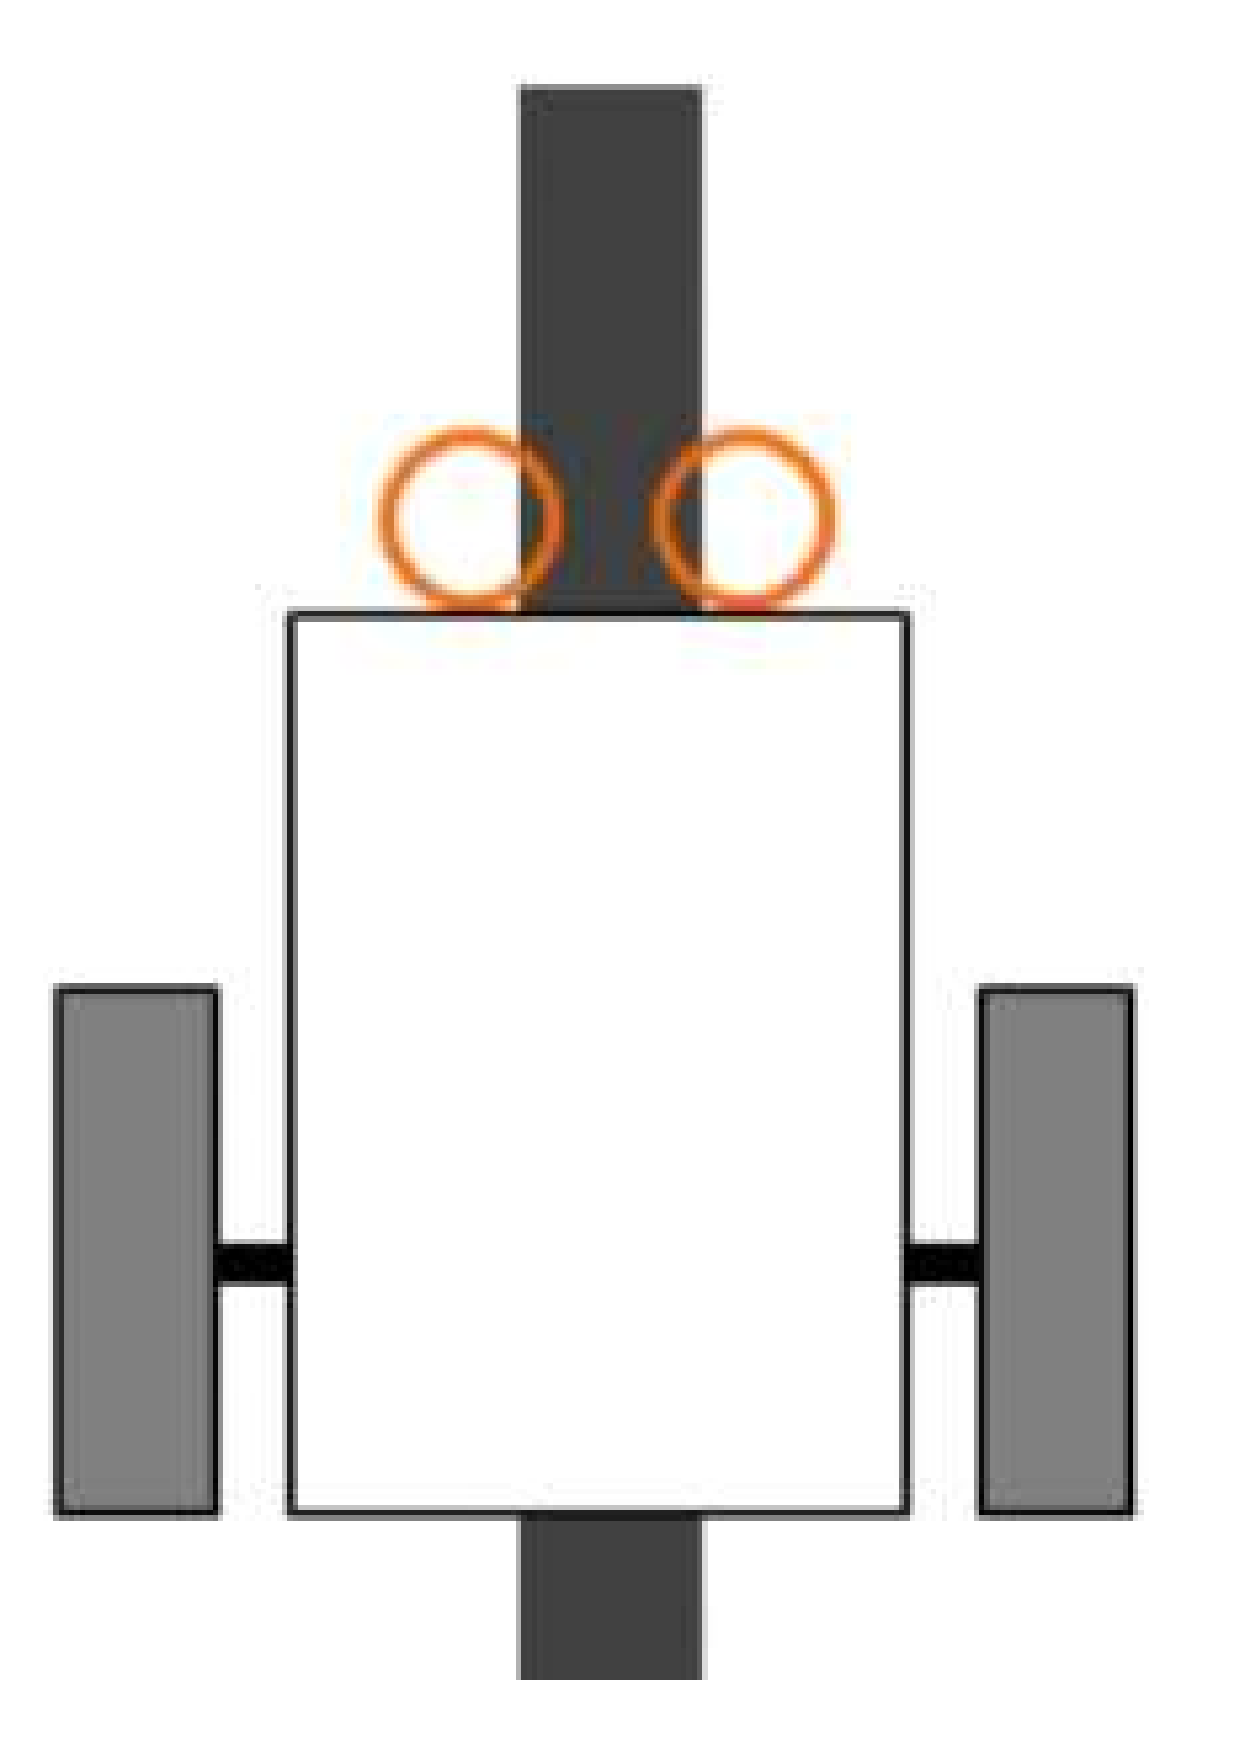
\includegraphics[scale=0.15]{sensor_1.pdf} \\ a)}
		\end{minipage}
		\hfill
		\begin{minipage}[h]{0.30\linewidth}
			\center{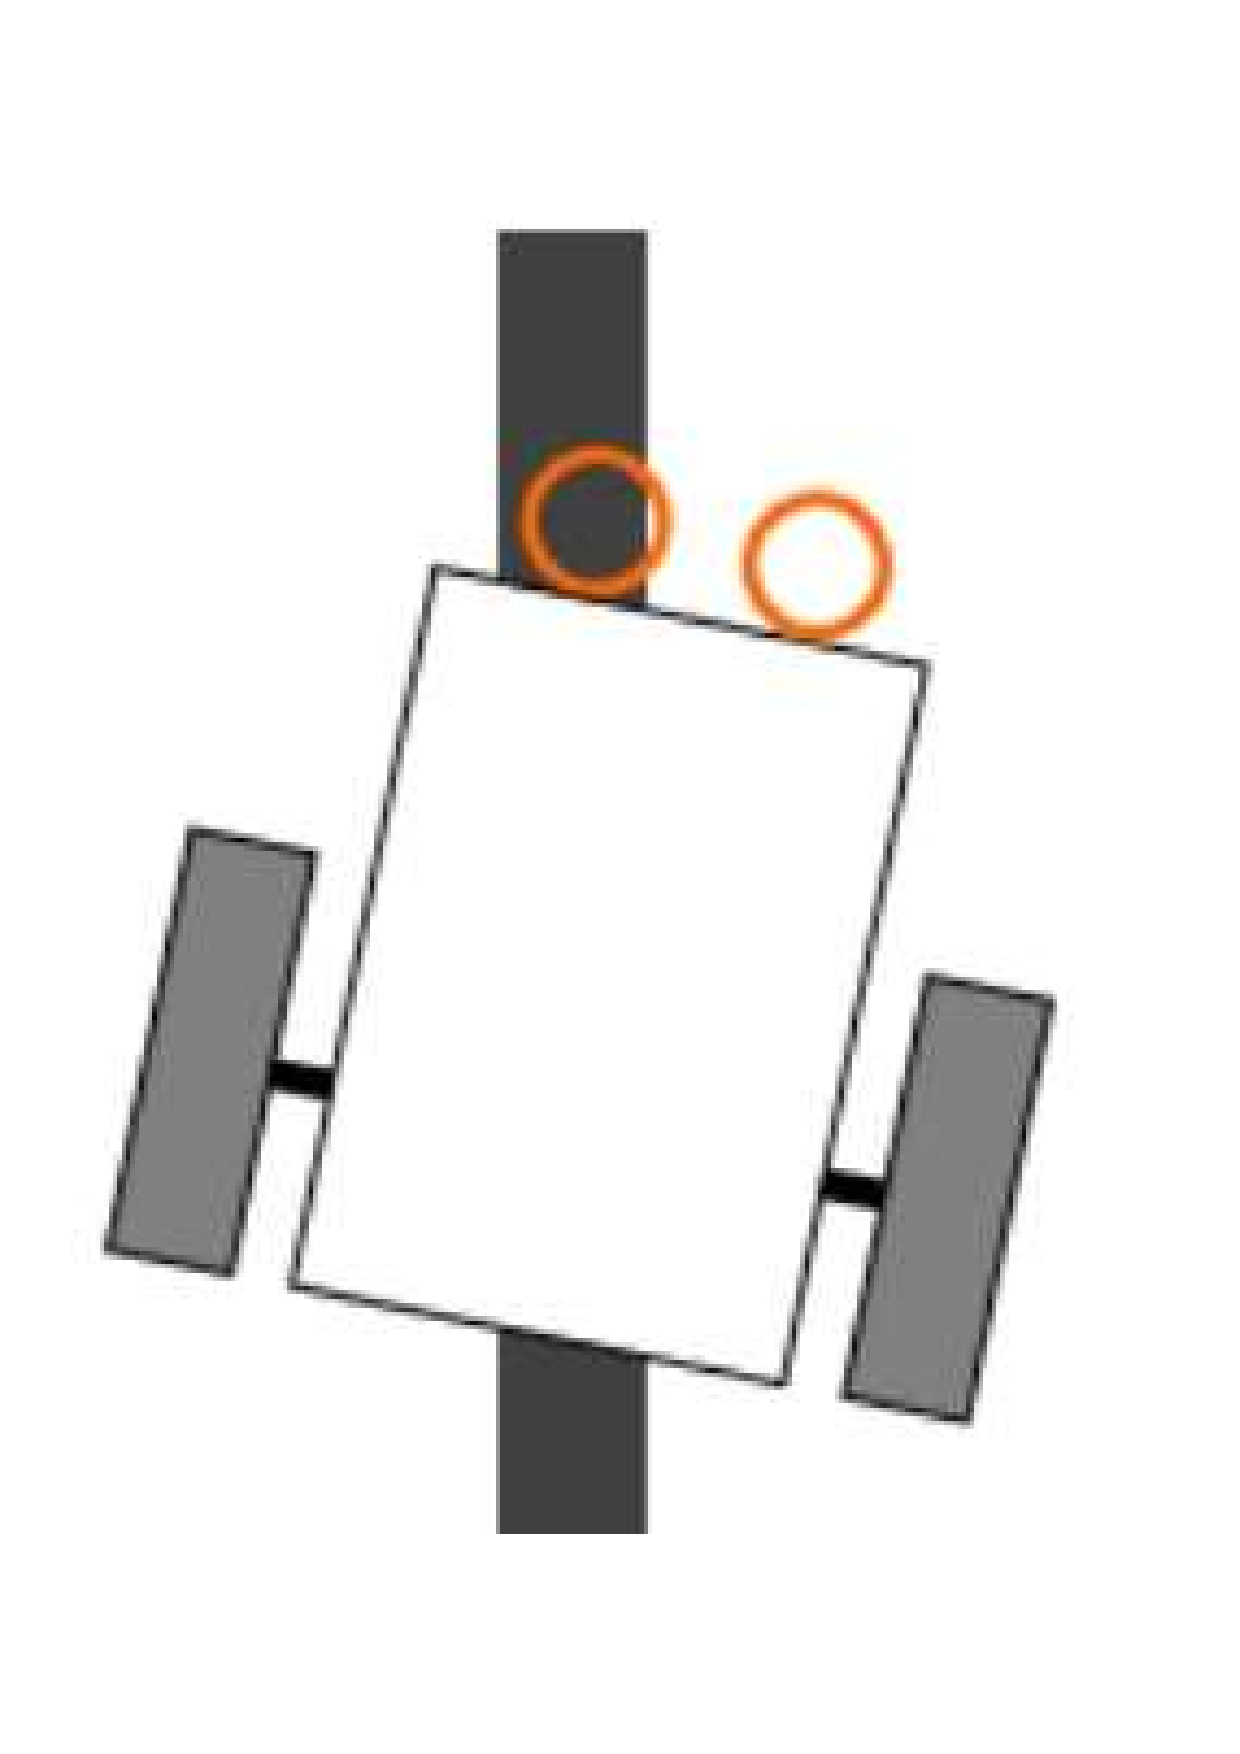
\includegraphics[scale=0.15]{sensor_2.pdf} \\ b)}
		\end{minipage}
		\hfill
		\begin{minipage}[h]{0.30\linewidth}
			\center{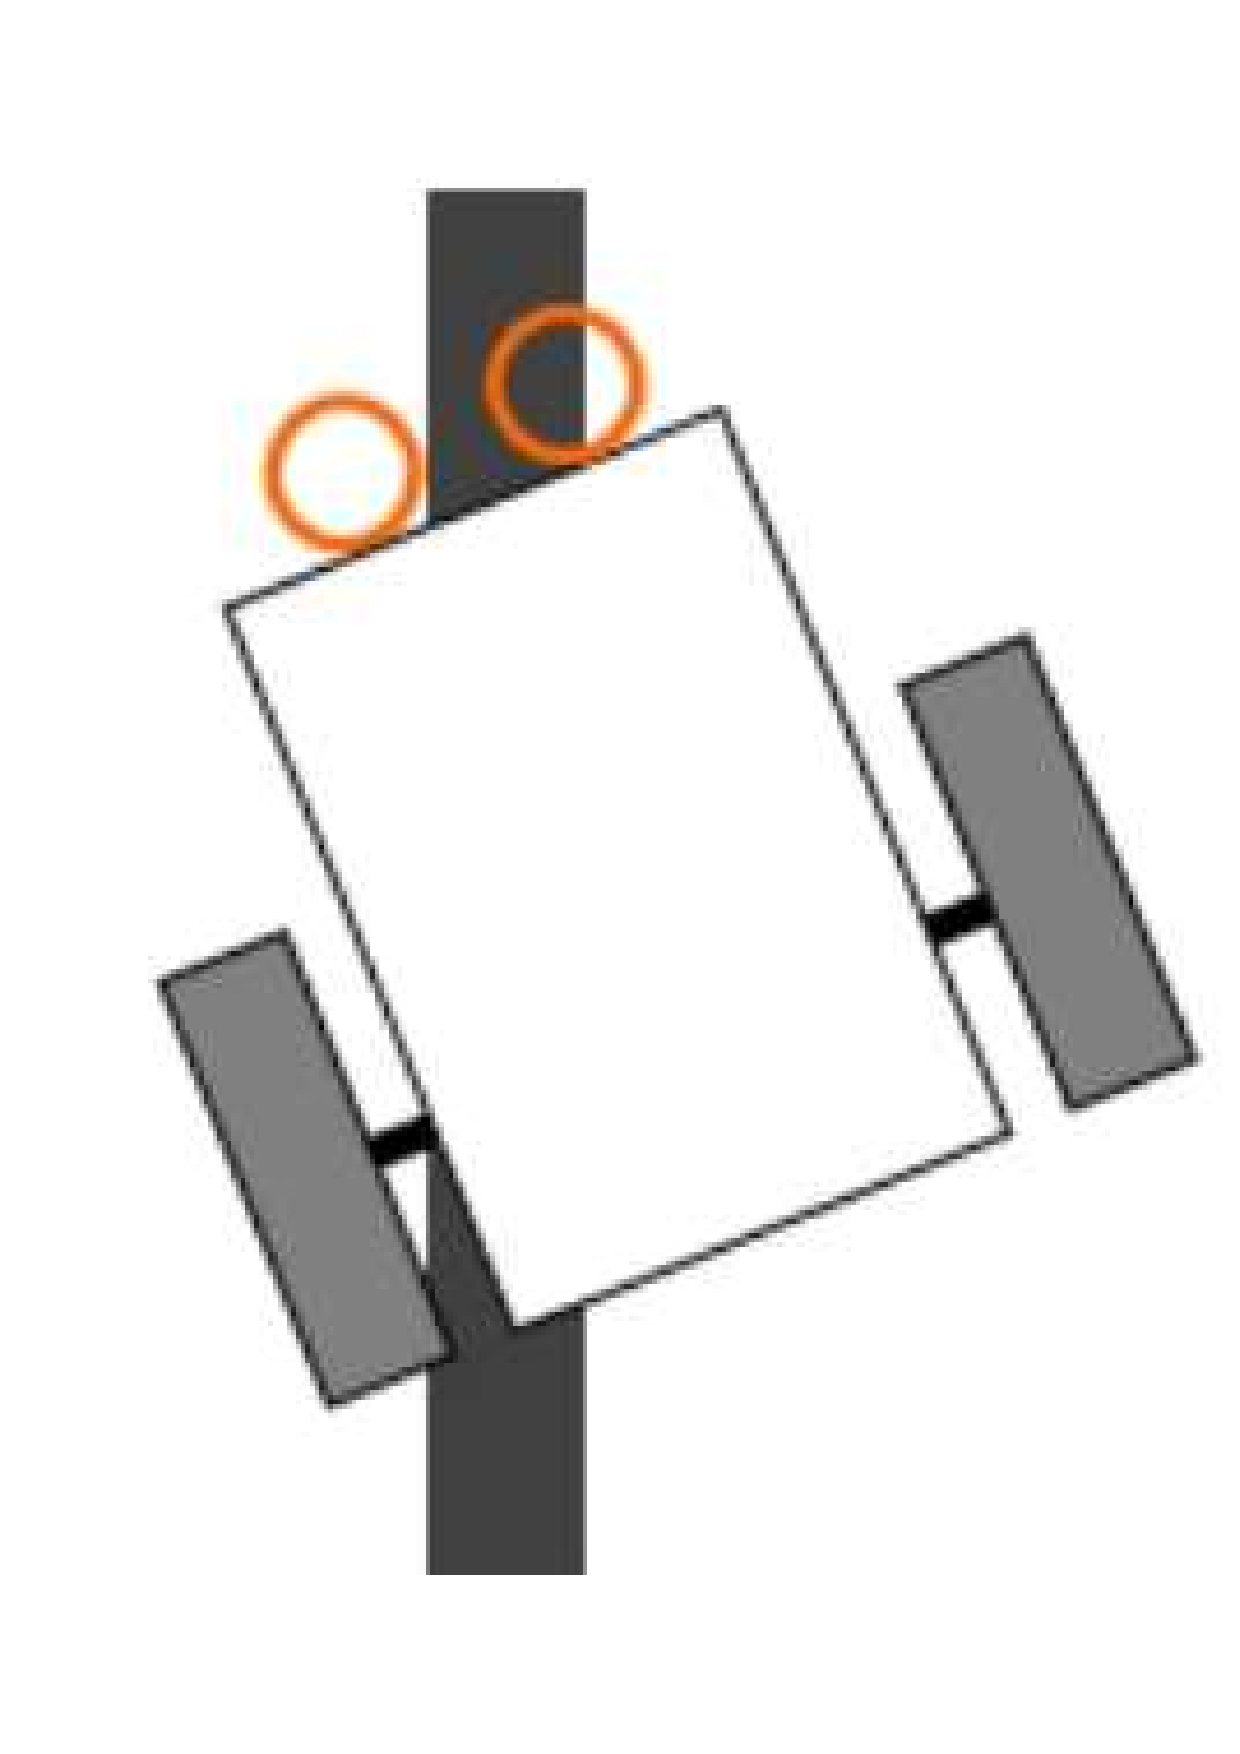
\includegraphics[scale=0.15]{sensor_3.pdf} \\ c)}
		\end{minipage}
		\caption{Sensors}
		\label{fig:sensor}
	\end{figure}


	We generalize two-light sensors approach on array of pixels, where the left and right sides of image represents left and right sensors respectively. The difference between these sides used as main control signal.  
	
	Whether a pixel belongs to a line is determined based on the fact that the surface surrounding the line significantly differs in color. Therefore, we use threshold binarization in order to determine belonging the current pixel to the line. Also binarization generate noise that approximately the same in the entire frame. However noise reduced, because resulting control signal depends on the difference of frame sides.
	
	To count each side weight we use distance of black pixels from central vertical line and  multiply it by two coefficients:
	
	\renewcommand{\labelenumii}{\arabic{enumii}.}
	
	\begin{enumerate}
		\item Camera perspective distortion correction (Affine transformation)
		
		\item Coefficient that reflect the distance from the vehicle. (farther away part of the line has smaller weight)
	\end{enumerate}
	
	\renewcommand{\labelenumii}{\arabic{enumi}.\arabic{enumii}.}
	
	The ideological structure of the project represents on figure \ref{fig:diagram}. The camera forms a frame and sends it to the FPGA pixel-by-pixel. During image transfer pixel-flow algorithm compute control signal. When the last pixel received, proportional regulator changes the control signal and send it to the motor driver. To control a motor power, we use pulse width modulation (PWM) technique. 
	
	\begin{figure}[h]
		\center{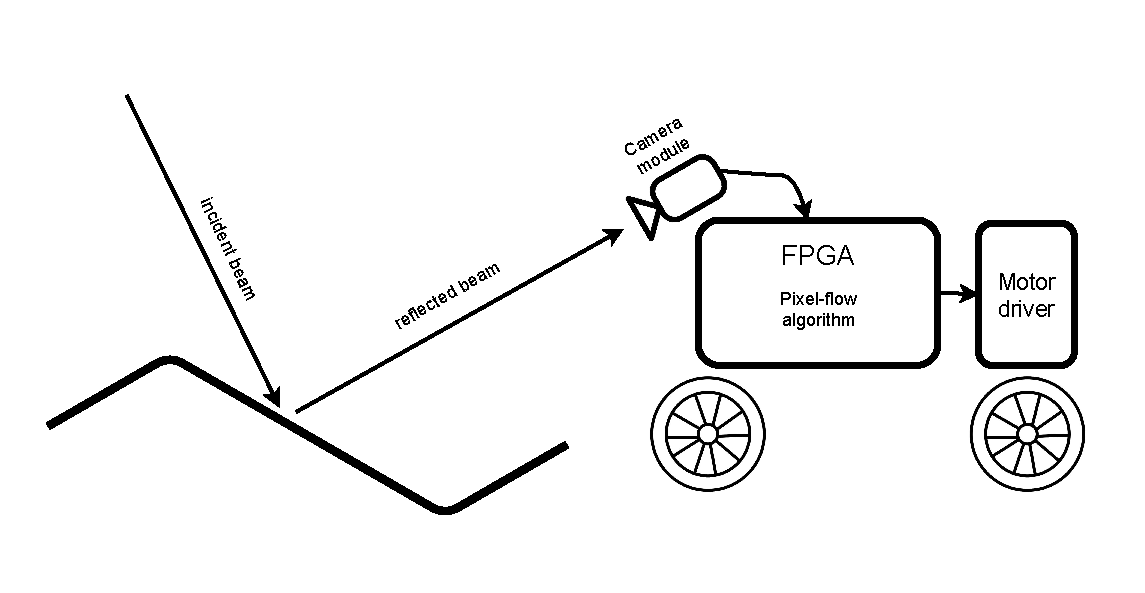
\includegraphics[scale=0.7]{Diagram.pdf}}
		\caption{image}
		\label{fig:diagram}
	\end{figure}
	
	\newpage
	The resulting vehicle control algorithm consist of following steps:
	\renewcommand{\labelenumii}{\roman{enumii}.} 
	
	\begin{enumerate}
		\item (Initialization) Set zero to the control signal registers
		\item Wait the frame receiving starts
		\item Receive the pixel and update pixel position
		\item Threshold pixel value 
		\item Compute camera perspective distortion and distance dependent coefficients
		\item Update control signal value \\ if current pixel the last go to step \romannumeral 7, otherwise \romannumeral 3
		\item Update control signal using proportional regulator
		\item Set control signal on motor driver
		\item Set zero to the control signal registers and go to \romannumeral 2  \hspace{5pt}step
	\end{enumerate}

	When we launch FPGA, it initialize camera communication protocol and resets coefficients registers to zero. As soon as camera is ready to send new frame, it rise high level signal on separate communication line. During frame pixel-by-pixel transferring FPGA determine belong current pixel either to left or right frame side and then compute coefficients and update control signal register. When frame transferring is finished, FPGA compute difference of frame-sides coefficients. Proportional regulator converts received difference into 8 bit value and sends it to the PWM module. 
	
	\renewcommand{\labelenumii}{\arabic{enumi}.\arabic{enumii}.}
	
	\vspace{8mm}
	
%	\begin{figure}[h]
%		\center{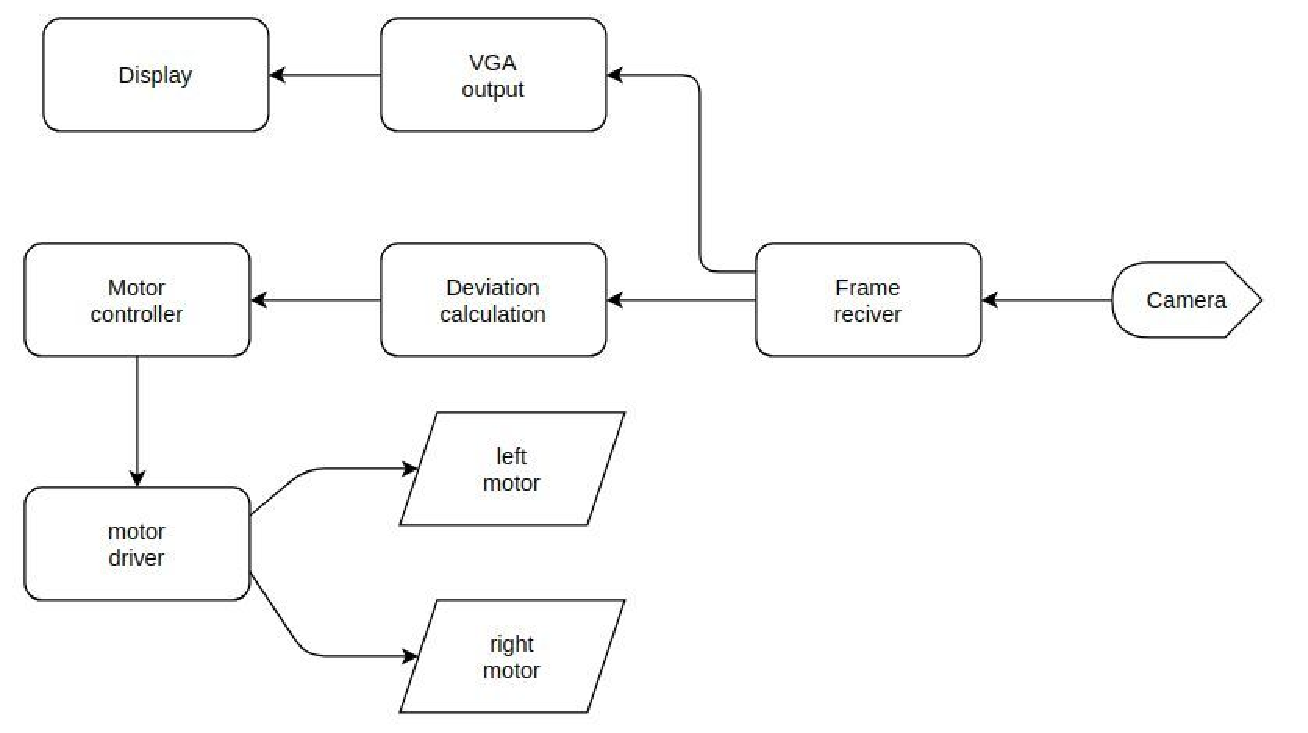
\includegraphics[scale=0.7]{im4.pdf}}
%		\caption{image}
%		\label{fig:im4}
%	\end{figure}
%
%	General project structure represents on the figure \ref{fig:im4}. Also you can see another data flow, that contains VGA output. It used for algorithm debugging. 

	\item \textbf{Algorithm math details}
	\begin{enumerate}
		\item Basis changing 
		
		To simplify computations coordinate system of pixels counter should be changed to another one based in middle of the lower boundary of the image. For pixel counting we use a coordinate system based in the top left corner of the image and y-axes pointing down, x-axes directed to the right. Equation \eqref{eq:sysChange} reflects the transition to a new coordinate system
	
		\begin{equation}
			\left\{
				\begin{aligned}
					x_{\text{new}} &= | \text{width\_of\_image} / 2 - x_0 | \\
					y_{\text{new}} &= -y_0\\
				\end{aligned}
			\right.
		\label{eq:sysChange}
		\end{equation}
	
	\begin{flushright}
		\footnotesize where $x_{\text{new}}$ and $y_{\text{new}}$ are coordinates in a coordinate system based in the center of the image bottom.
	\end{flushright}
	


	\newpage
		\item Affine transformation
		
		The camera inclination leads to occurrence of perspective distortion. To correct perspective distortion we use affine transformation. The influence of affine transformation shown on figure \ref{fig:affine}, where figure  \ref{fig:affine}.b the result of correction of \\figure \ref{fig:affine}.a.
		
		\begin{figure}
			\begin{minipage}[h]{0.49\linewidth}
				\center{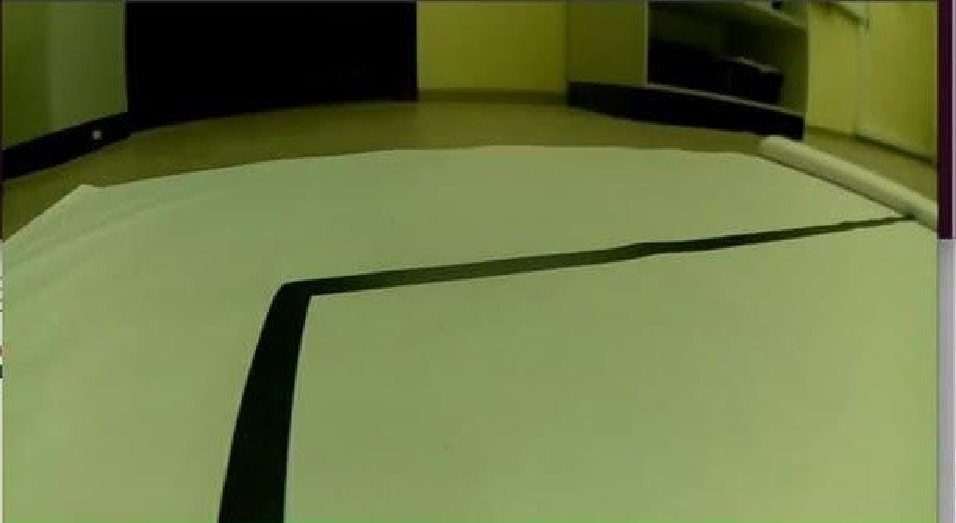
\includegraphics[scale=0.7]{im5.pdf} \\ a)}
			\end{minipage}
			\hfill
			\begin{minipage}[h]{0.49\linewidth}
				\center{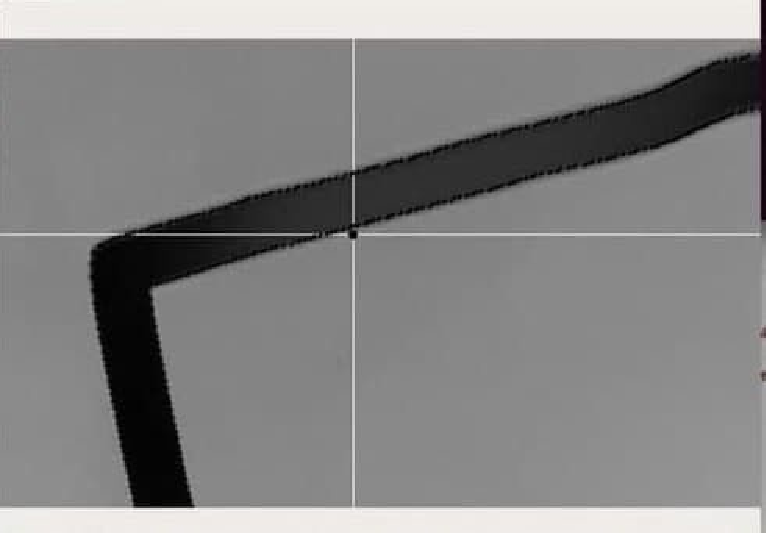
\includegraphics[scale=0.7]{im6.pdf} \\ b)}
			\end{minipage}
		
		\caption{Affine}
		\label{fig:affine}
		\end{figure}

		\hspace{0.05cm}

		In our case transformation shapes: isosceles trapezoid to rectangle, where the bases of the trapezoid are parallel to the bottom of the frame. Therefore we have the simplest case of transformation, where the bottom base of the trapezoid is almost two times bigger than the upper base. In more complex cases, transformation shape can represent an arbitrary convex quadrilateral. We can compute distortion coefficient of the each pixel using the following formula: 

		\hspace{0.1cm}

		\begin{equation}
			\left (
			1 + \frac{y}{430}
			\right )
		\end{equation}

		\begin{flushright}
			\footnotesize where 430 is height of our image.
		\end{flushright}

		\newpage

		\item Deriving deviation coefficient
		
		Also we introduce a coefficient that reflect the distance of the line segment from the vehicle. Empirically it was found that the exponential function with a range of coefficients from 1 to 0.3 is most effective, where 1 and 0.3 refer to bottom and top respectively. For computing exponential function on FPGA we use Maclaurin series:

	%	\hspace{4mm}

		\begin{equation}
			e^x = 1 + \frac{x}{1!} + \frac{x^2}{2!} + \ldots + \frac{x^n}{n!} + \ldots = \sum\limits_{i=1}^{\infty} \frac{x^n}{n!} \text{, } |x| < \infty
		\end{equation}
		

		with sufficient accuracy, we can only use the first four terms.
		%\vspace{6mm}
		
		Deviation coefficient formula:

		\begin{equation}
			m(x) = 1 - \left ( \frac{x}{405}\right) + 
			\frac{\left ( \frac{x}{405}\right) ^2}{2}  -
			\frac{\left ( \frac{x}{405}\right)^3}{6}
		\end{equation}

		\begin{flushright}
			\footnotesize Coefficient “405” is used for values normalization \\
			$e$( 0.3, 1 ) to x( -1.066, 0 ), 430 = 405*1.066
			
		\end{flushright}
		\vspace{1cm}
		
		%\section*{Resulting coefficients formula}
		\item Resulting coefficients formula
		
		Equation \eqref{resFormula} represents the resulting formula for affine transformation and deviation correction coefficients.

		\begin{equation}
			\left ( 1 + \frac{y}{430}\right )
			\left (  
			1 - \left ( \frac{x}{405}\right) + 
			\frac{\left ( \frac{x}{405}\right) ^2}{2}  -
			\frac{\left ( \frac{x}{405}\right)^3}{6}
			\right )
			\label{resFormula}
		\end{equation}
		\vspace{1cm}
		
		\item The choice for algorithm parameters
		
		Since Verilog HDL is hardware description language it does not have effective division operator. To overcome this challenge we replace division by shifting operator. Example of replacing is shown below:
		
 
		
		\begin{align*}
			\frac{1}{43} &\approx 0,02326 \\
			[A] &\text{ - rounding to nearest integer} \\
			\frac{1}{43} &= \frac{2^n}{43 \cdot 2^n} \approx \frac{\left [ \frac{2^n}{43} \right ]}{2^n} \\  \\
			&\text{example: } n = 7\\
			\frac{2^7}{43} &\approx 2,9767 \approx 3 \Rightarrow 
			\frac{1}{43} \approx \frac{3}{2^7} \\
			\frac{3}{2^7} &\approx 0,02362
		\end{align*}
		
		The second challenge is normalizing the difference of frame's sides before sending it to the proportional regulator. To evaluate the required size of the register we compute the maximum side coefficient value:
		
		%The first step is evaluating the maximum value that can be reached. 
		%To get this value, we have to calculate area under graph shown on figure 10 that equal the double integral over our surface.
		
		\begin{equation}
		\begin{aligned}
			\int_0^{430} \int_0^{320} 
			\left ( 1 + \frac{y}{430}\right )
			\left (  
			1 - \left ( \frac{x}{405}\right) + 
			\frac{\left ( \frac{x}{405}\right) ^2}{2}  -
			\frac{\left ( \frac{x}{405}\right)^3}{6}
			\right )
			&x
			dx
			dy\\
			&\approx 1,96968 \times 10^7 
		\end{aligned}
		\end{equation}
		
		%This value is also needed to determine the size of the register, in our case it is 25:
		\vspace{1cm}
		Required register size:
		
		\begin{equation}
			\log_{2}19696800 \approx 24,23 \Rightarrow 25
		\end{equation}
		
		\vspace{5mm}
		
		For normalization of coefficients values we use the following algorithm:  
		
		\begin{enumerate}
			\item 
			Shift to the right by 16 bits: (0;19696800) $\Rightarrow$ (0;300)
			
			\item 
			limit the value to 255 if it exceeds
		\end{enumerate}
		
		\newpage
		
		\item Motor controller
		\vspace{5mm}
		
		Motor controller module represented by proportional regulator and  PWM modules.
		The motor controller perform two main operation:
		
		\begin{enumerate}
			\item Received control signal is changed by proportional regulator. 
			
			\item PWM module generate control signal that is fed to motor driver.  
			
		\end{enumerate}
	
		In order to get a stable work of the algorithm should be noticed some environment parameters such as width of the line, lighting, power of the motors and vehicle inertia. Therefore  proportional regulator is used for tuning the sharpness of algorithm and to handle environment parameters issues.
		
	\end{enumerate}
\end{enumerate}

\section*{Implementation}
\noindent In our project we employ following devices and software tools:
\begin{enumerate}
	
	\item 
	Cyclone \RomanNumeralCaps{4} FPGA board based on Altera EP4CE6E22C8N chip of low-cost and low-power Cyclone \RomanNumeralCaps{4} FPGA device family. The board appearance shown on figure \ref{fig:im1}
	
	\begin{figure}[h]
		\center{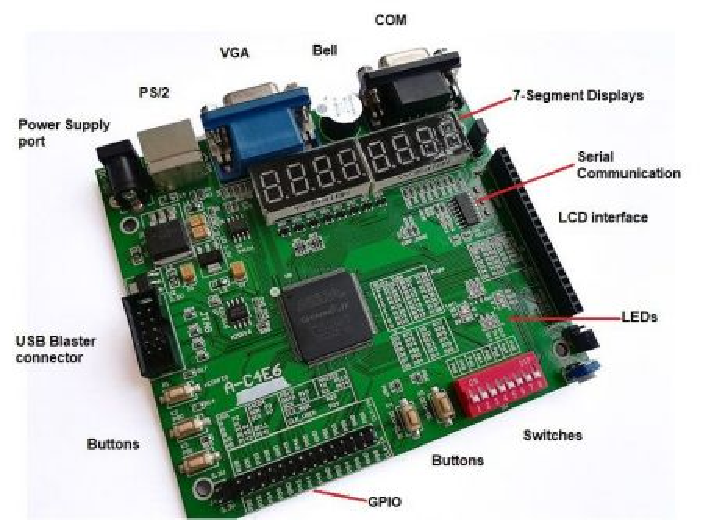
\includegraphics[scale=0.7]{im1.pdf}}
		\caption{image}
		\label{fig:im1}
	\end{figure}
	
	
	\item
	OV7670 Camera module based on  single-chip VGA camera and image processor in a small footprint package. It has resolution 640x480 and 8-bit serial bus for image transferring, providing up to 30 frames per second. Camera appearance shown on figure \ref{fig:im2}.
	
	\begin{figure}[h]
		\center{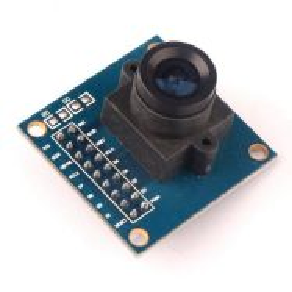
\includegraphics[scale=0.8]{im2.pdf}}
		\caption{image}
		\label{fig:im2}
	\end{figure}
	
	\item
	Motor driver L298N. It has 2 pins to direction control and one speed control pin each of two motor output. Appearance of driver shown on figure \ref{fig:im3}.
	
	\begin{figure}[h]
		\center{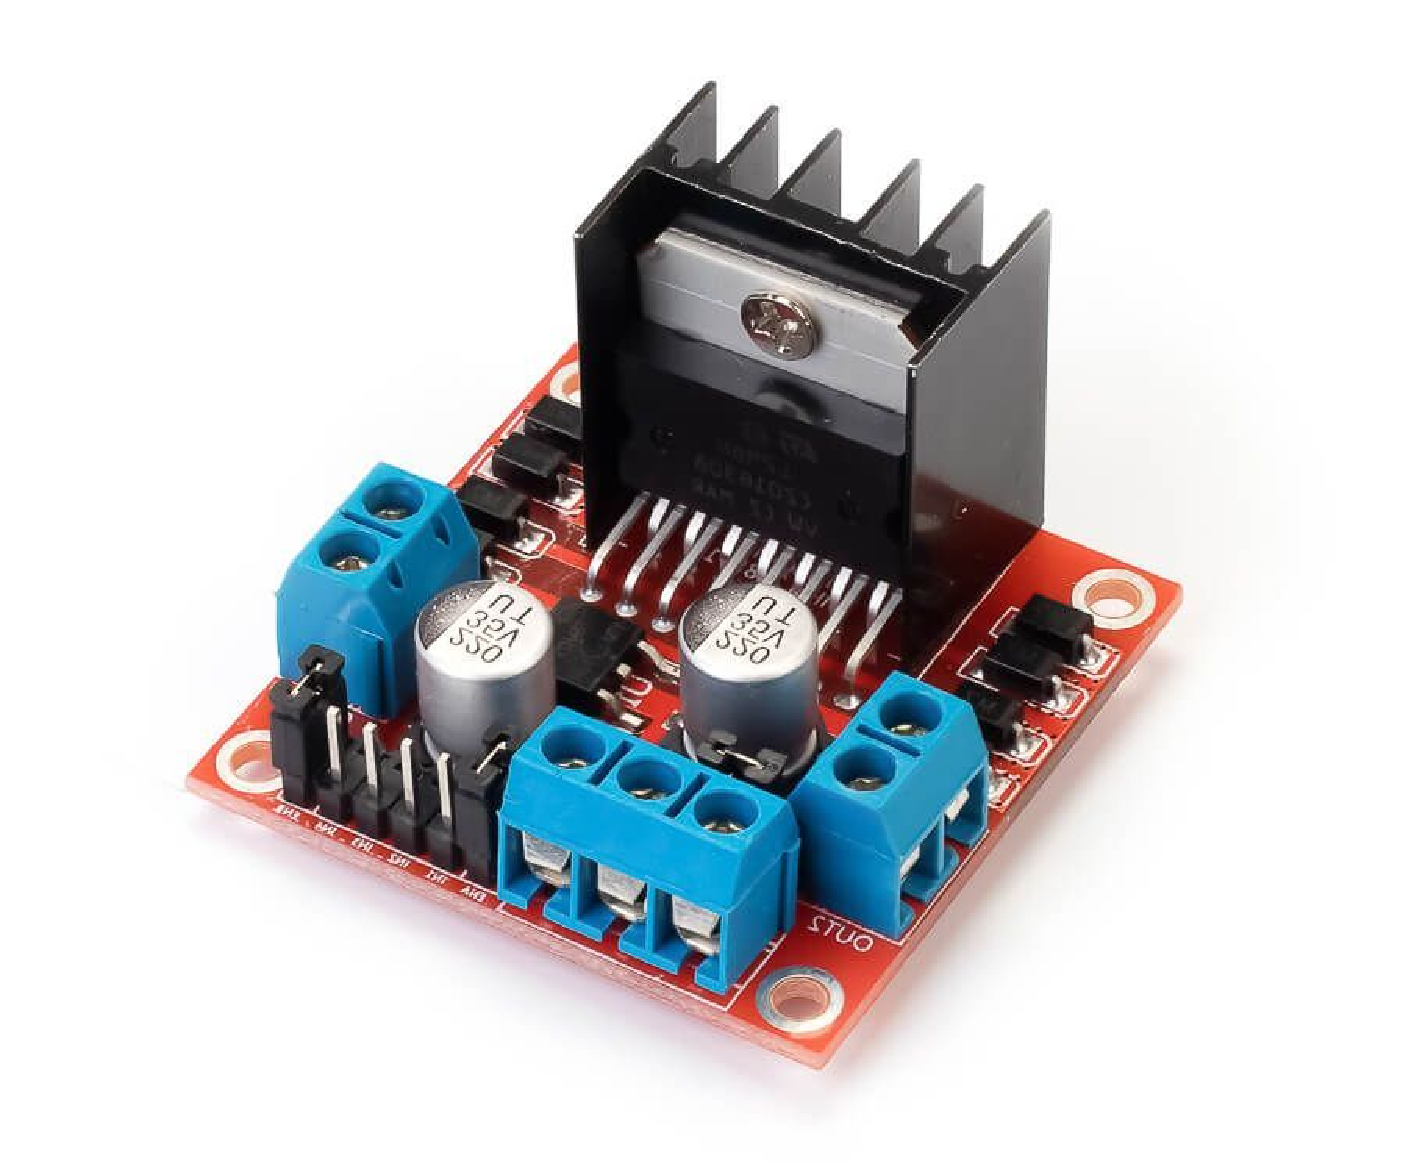
\includegraphics[scale=0.3]{im3.pdf}}
		\caption{image}
		\label{fig:im3}
	\end{figure}
	
	\item 
	Software development environment Intel Quartus Prime 20.1V (Lite Edition). Program developed on Verilog HDL programming language. Verilog HDL is one of the Hardware Description Language that uses modules as basic blocks for schematic description.
\end{enumerate}

\newpage
The appearance of the vehicle is shown in the figure \ref{fig:vehicle}.

\begin{figure}[h]
	\center{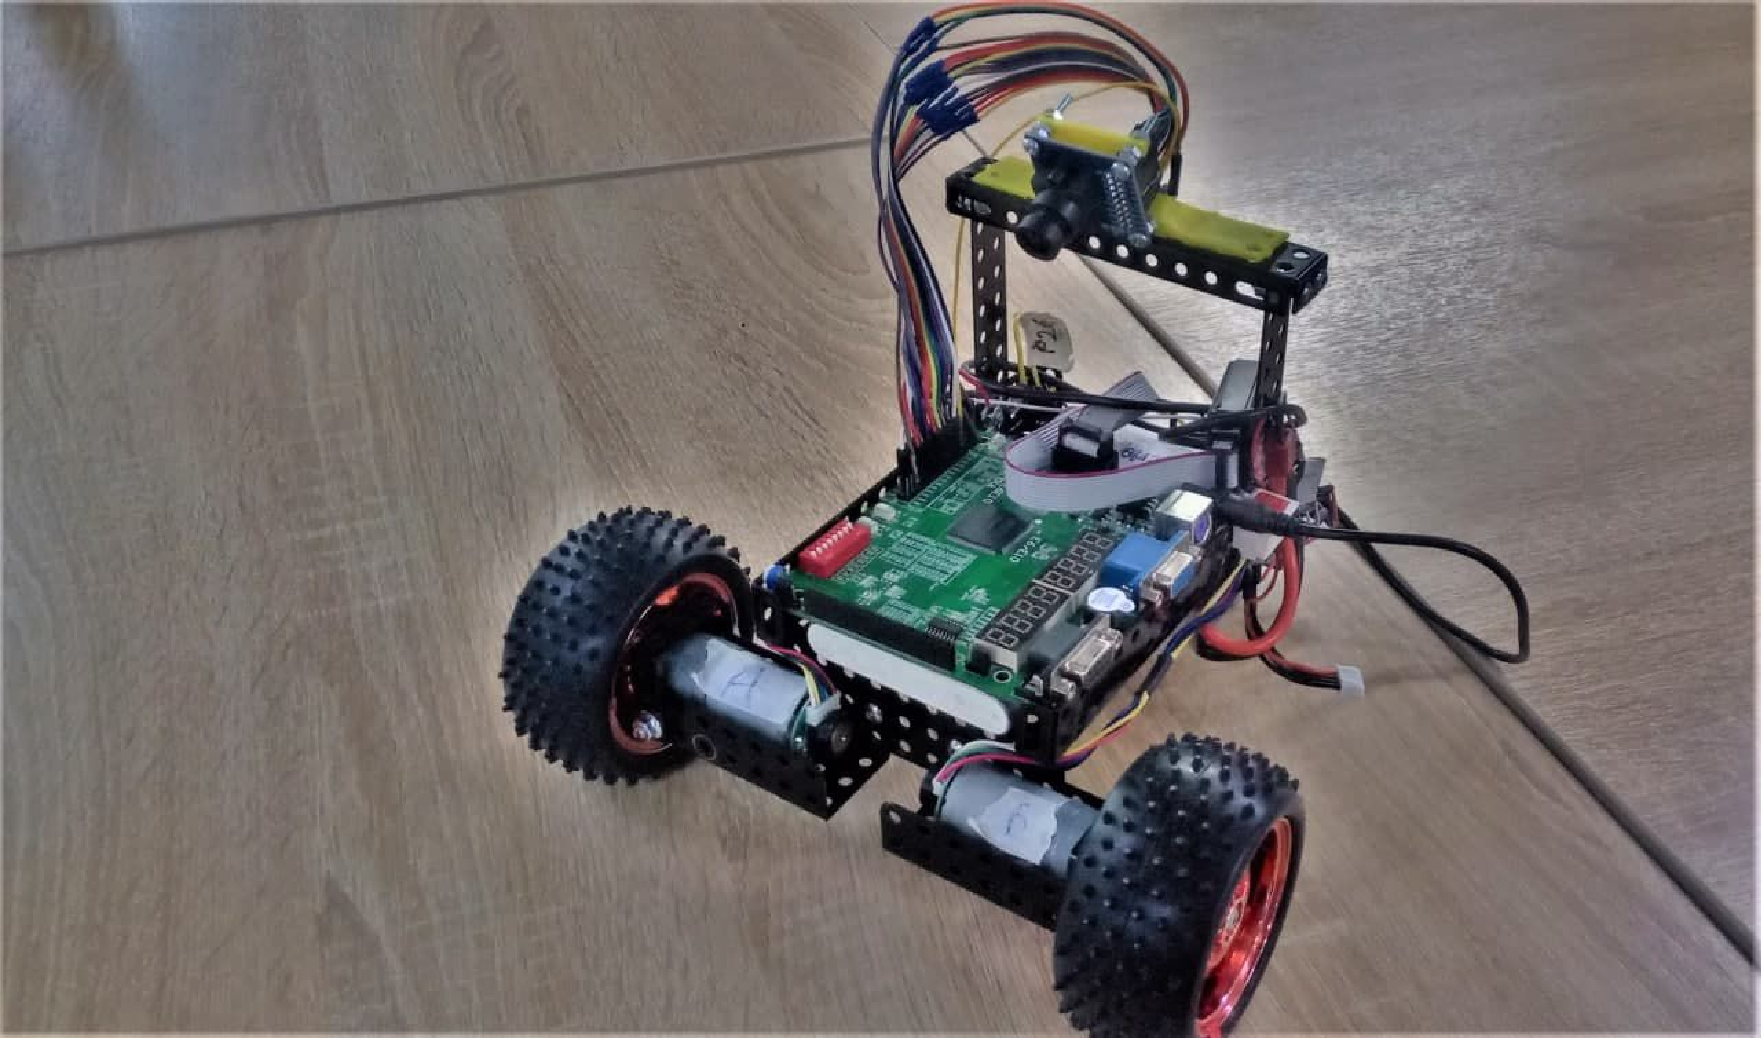
\includegraphics[scale=0.5]{vehicle.pdf}}
	\caption{image}
	\label{fig:vehicle}
\end{figure}

\newpage

\section*{Evaluation}

Derived algorithm was tested using two types of tags shown on figure \ref{fig:lines}. First type are represented on figure \ref{fig:lines}.a. The only restriction on this type is the next tag should lie in the camera view angle. The size and distance between tags depend on vehicle configuration. The figure \ref{fig:lines}.b represent example of continuous tags that also can be used for vehicle direction. The maximum curvature of the trajectory is determined from the required speed of movement and the inertia of the vehicle. 

\begin{figure}
	\begin{minipage}[h]{0.49\linewidth}
		\center{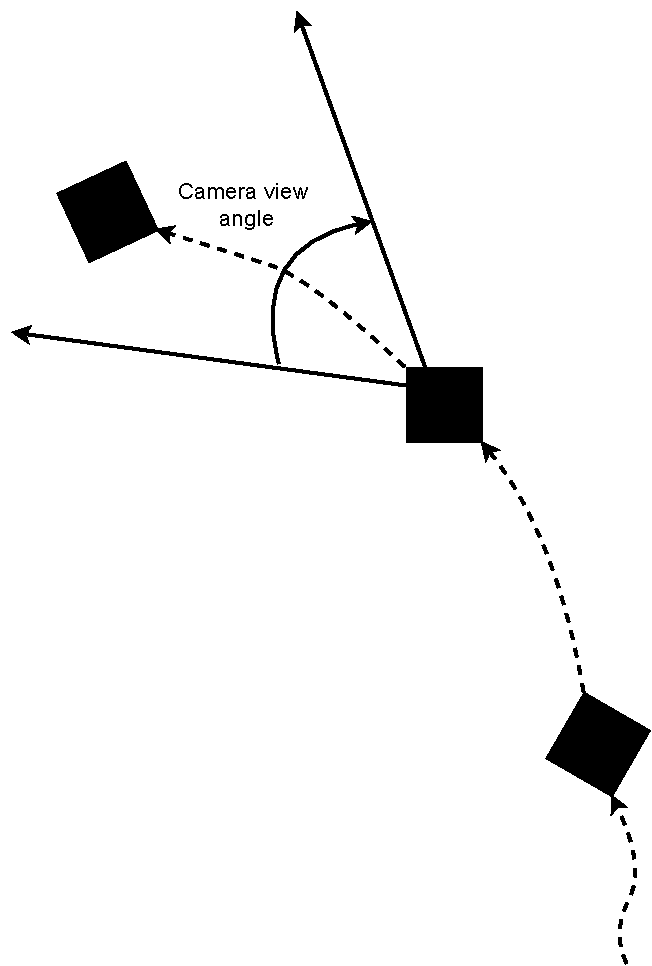
\includegraphics[scale=0.5]{line.pdf} \\ a)}
	\end{minipage}
	\hfill
	\begin{minipage}[h]{0.49\linewidth}
		\center{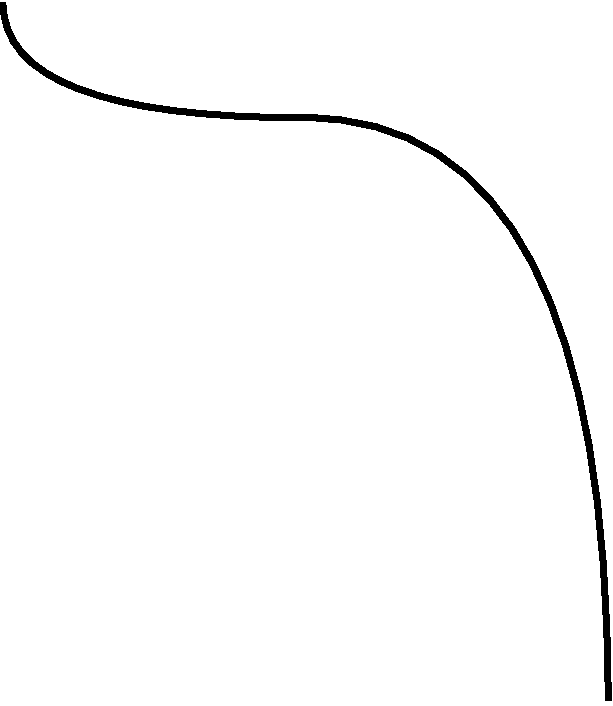
\includegraphics[scale=0.65]{lineCont.pdf} \\ b)}
	\end{minipage}
	
	\caption{types of guide marks}
	\label{fig:lines}
\end{figure}

Also, to assess the resource consumption of the algorithm, we compiled the pixel processing module separately. Required number of logical units for algorithm processing is 338. Cyclone \RomanNumeralCaps{4} FPGA has 6,272 logical units, hence the amount of resources spent is about 5 percents.




\section*{Future improvements}  

One of the main algorithm parameter is the binarization threshold. It depends on the color of line, lightning and sensitivity of the camera. We going to implement additional algorithm in order to automatize threshold determining. An algorithm may use first few frames for computing stable threshold value. 

Also, due to the pixel processing is done independently, it possible to handle several pixels simultaneously. The throughput of this approach will be determined from the number of parallel processing branches. To implement this idea, we also need to create a queue for incoming pixels. 


\section*{Conclusion}

Developed algorithm based on the assumption that    

\end{document} % конец документа